\section{Near-Field Model}
\label{sec:near_field_model}

\subsection{Conceptual model and geometry}
In order to capture key transport domains in the scale of single access tunnel,
we consider a~computational geometry comprising the disposal wells $\Omega_w^i$,
where the \Gls{WDP}s will be stored, the access tunnel with backfill $\Omega_b$,
excavation influence zone $\Omega_e$, intact rock $\Omega_r$, and a fault zone
$\Omega_f$, see \figref{fig:conceptual}. The fault zone $\Omega_f$ located
close to the downstream boundary is represented as a discrete fracture extending
vertically across the entire computational domain and acting as a hydraulic
conductor connecting to the top and bottom boundary planes used for the
evaluation of \gls{QoI}.

 Where applicable, the dimensions follow the technical solution of DGR
 % \cite{HausmannovaTechnicke2023}.
  \cite{HausmannovaTechnicke2025rev}
  % \cite{HausmannovaTechnicke2025rev}.

\begin{figure}[htb]
\centering
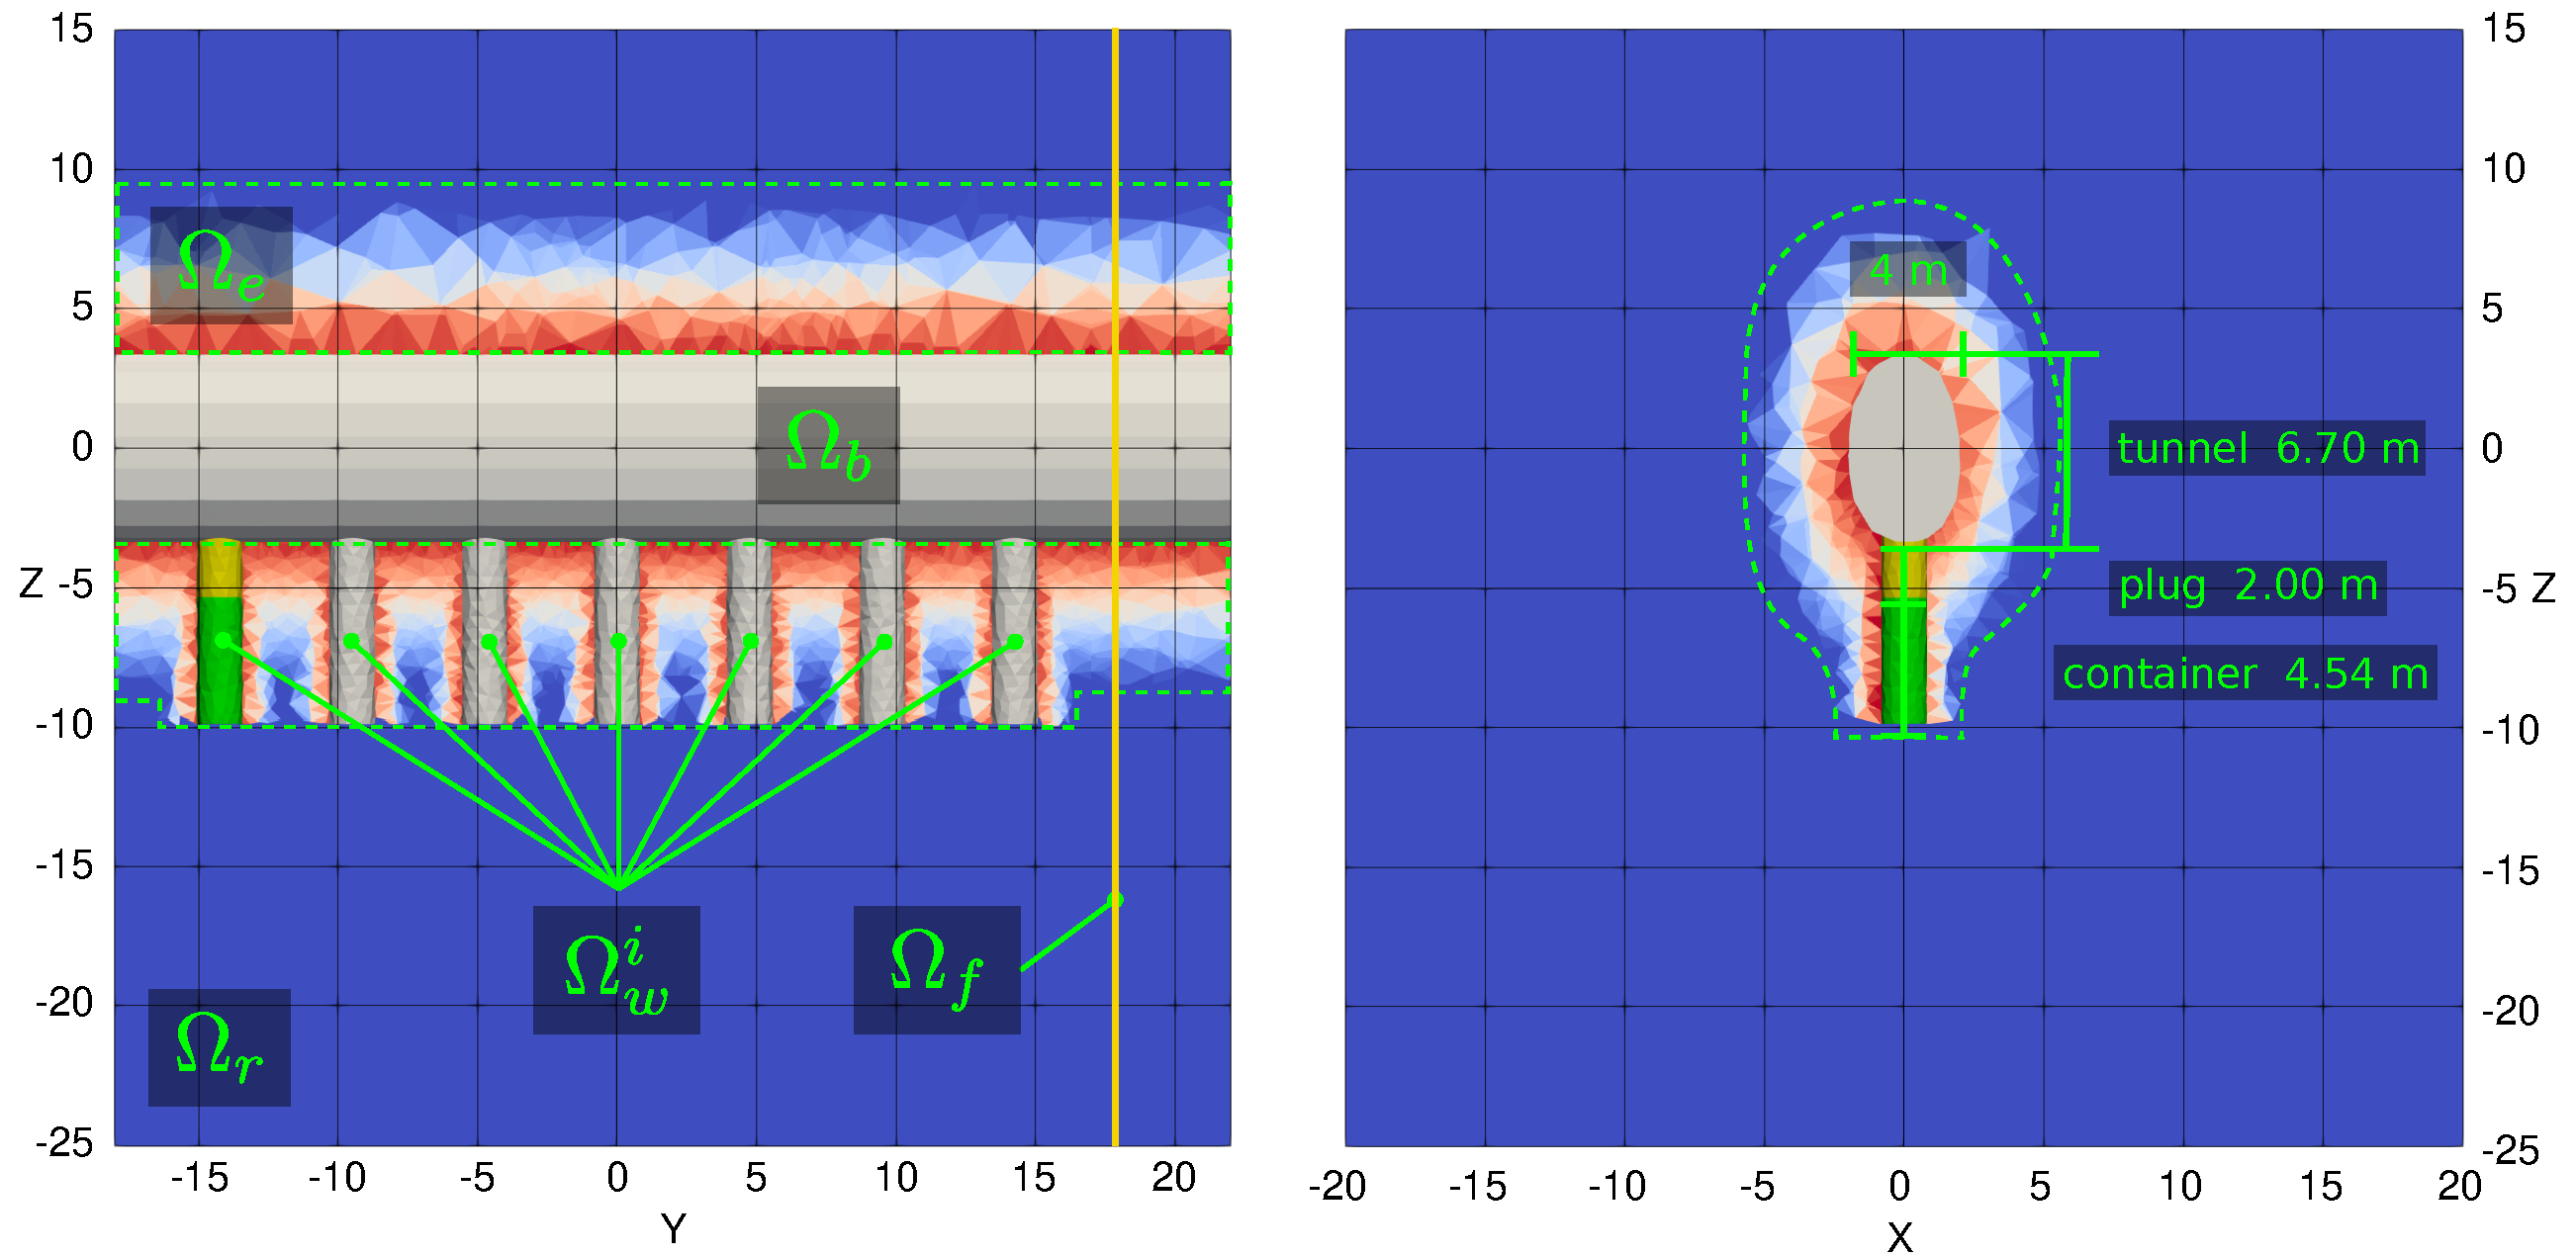
\includegraphics[width=\textwidth]{graphics/tr/cond_cut_edit.pdf}
\caption{Computational domains cuts in $xz$ and $yz$ planes domain with
hydraulic conductivity field denoting the extent of the EDZ. Fractures are
omitted.}
% TODO: smaller latex font
% \caption{TODO: Cut through the transport domain with fractures and permeability field denoting the extent of the EDZ}
\label{fig:conceptual}
\end{figure}

The disposal wells $\Omega_w^i$, $i=0,\dots, 6$, are represented by cylinders
with dimensions following the \gls{WDP} design for VVER-440 waste. Dimensions
are, diameter $d_w=1.65\munit{m}$ and height $h_w=6.54\munit{m}$, including the
$b_w=2\munit{m}$ spacer block. The actual waste package is not resolved, but
the volumetric contamination source $f_w$ $\bunit{m^{-3}\cdot s^{-1}}$ is
prescribed in the \gls{WDP} part below the spacer block. The source term is
only applied to the most upstream well, $31\munit{m}$ from the fault zone. The
volumetric source is proportional to the concentration difference over the
whole volume of the source well:

\begin{equation}
\label{eq:pulse_source}
    f_w = \alpha_w\big(c_w(t) - c(t, \vc x)\big)
    \qquad \text{on $\Omega_w^0$}.
\end{equation}
To simplify interpretation of the results, we assume a
unit 50-year concentration pulse in the waste package:
\[
c_w(t) = \chi_{(0,50)}(t).
\]
% c_w(t) ... bude jednickovy pulz v prvnim kroce 0-30 y

The coefficient $\alpha_w$ reflects the diffusion through the bentonite buffer:
\[
 \alpha_w = \frac{D_b}{ w}\frac{S}{V},
\]
where $D_b$ $\bunit{m^2\cdot s^{-1}}$ is the diffusion coefficient of
bentonite, $w=0.368\munit{{m}}$ is the buffer thickness,
$S\approx 12.36 \munit{m}^2$ is the waste package surface
(with $r=\frac{d_w}{2} - w=0.914\munit{m}$,
$h=3.79\munit{m}$) and $V=2.97\munit{m^3}$
% PE:
% S = 0,914×3,79×3,14256 + 2*3,14256*0.25*0,914 = 12,32 m2
% V=4,54×0,25×3,14256×0,914×0,914 = 2,97 m3
is the whole source domain volume.
The buffer thickness above \gls{WDP}, $0.4\munit{m}$, and below,
$0.35\munit{m}$, is approximated by $w$ for simplicity.




 All the well domains  $\Omega_w^i$ have transport properties common with the
access tunnel domain $\Omega_b$ corresponding to the transport properties of
the bentonite. The access tunnel $\Omega_b$ has a simplified smooth profile
resulting from averaging the laserscan data from tunnels at \URFB
and vertically scaled to the design dimensions: height $6.7\munit{m}$, width
$4\munit{m}$. Excavation of the access tunnel leads to increased permeability
in the excavation disturbed zone $\Omega_e$. Original idea to use posterior
data from inversion of the pore pressures experiment could not be implemented
due to complex rock structure. The complex excavation induced changes in the
transport properties were simplified to the geometrical interpolation between
the maximal EDZ permeability $k_e$ and the permeability $k_r$ of the intact
rock on the domain $\Omega_r$ over the thickness of the EDZ $w_e$. See the
histogram of hydraulic conductivity over mesh elements in
\figref{fig:cond_histogram}. 
\jb{TODO: move conductivity hustogram and its discussion to the parametrization section}

The \Gls{DFM} approach combining
a~heterogeneous continuum and a~stochastic \Gls{DFN} is applied in both rock
domains $\Omega_e$ and $\Omega_r$. A~single major fault zone, represented by
a~vertical fracture crossing the whole domain, is placed at the downstream end
of the computational domain (vertical orange line in \figref{fig:conceptual}
left). It effectively transports contamination to the (bottom) boundary where
the safety indicator is evaluated.

\begin{figure}[htb]
\centering
% 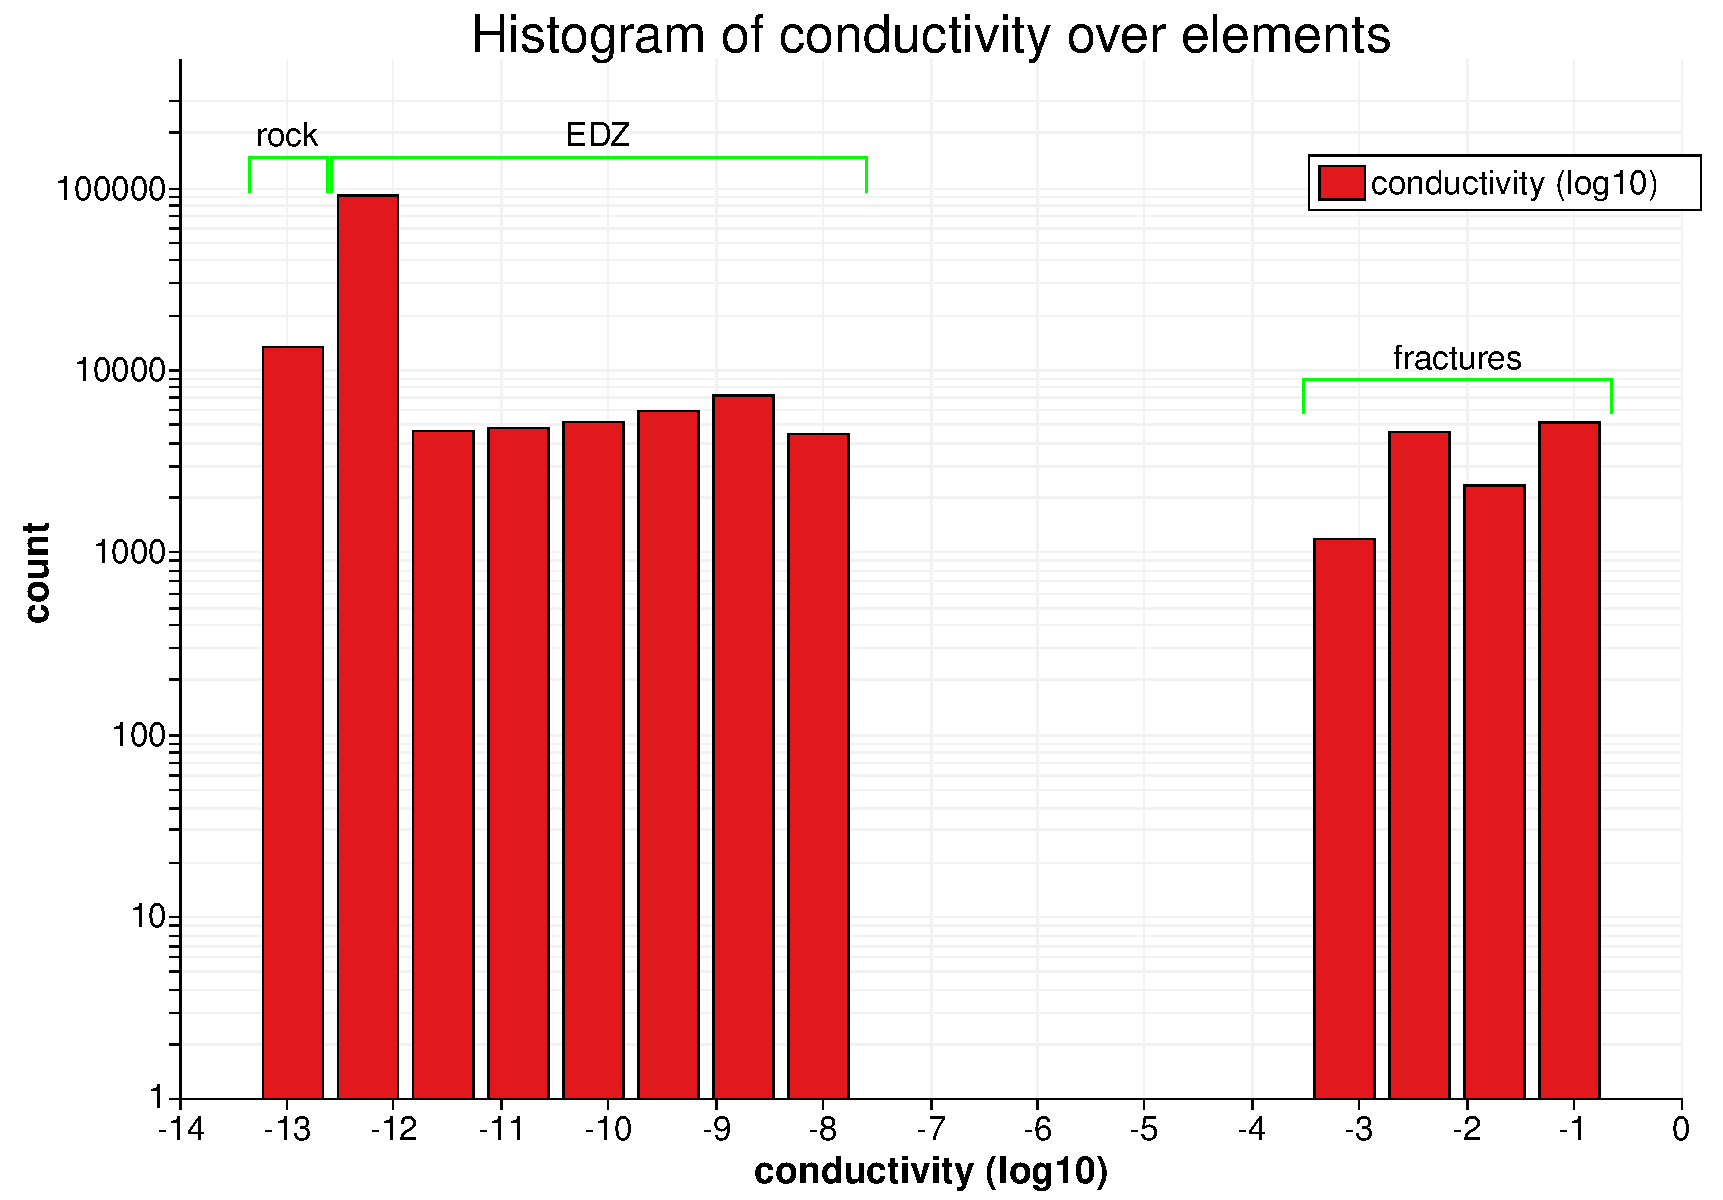
\includegraphics[width=0.75\textwidth]{graphics_tr/conductivity_hist_001_edit.pdf}
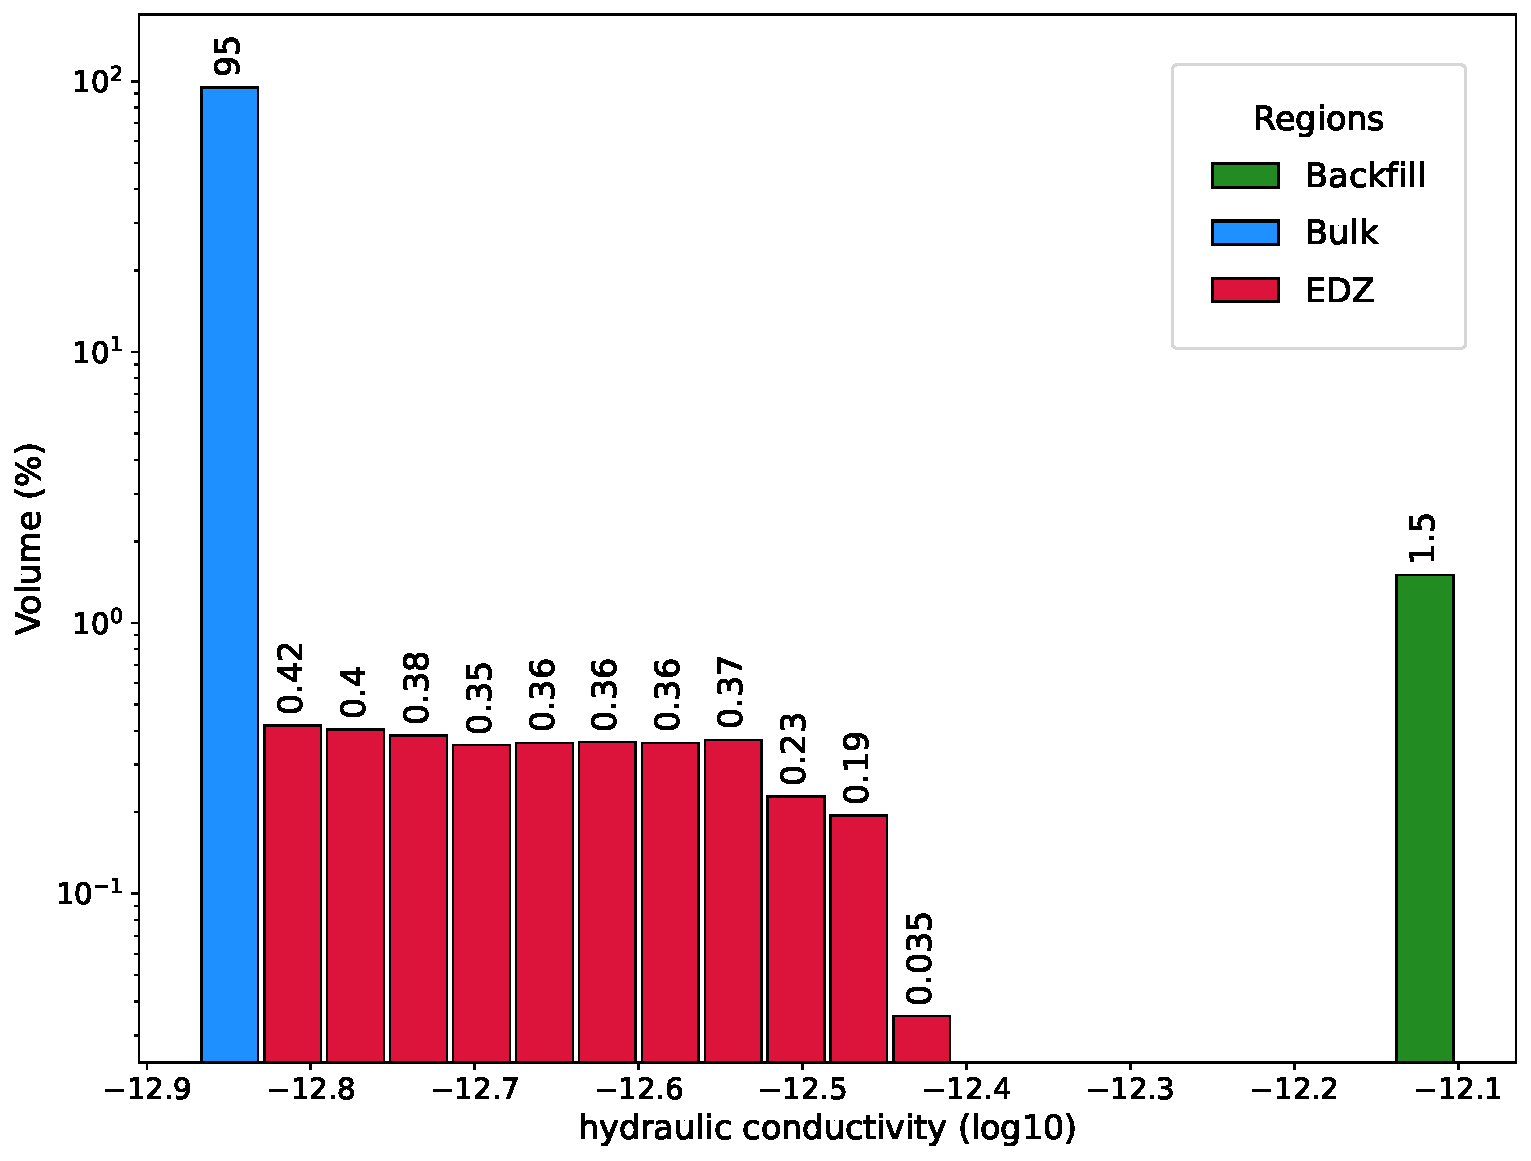
\includegraphics[width=0.75\textwidth]{graphics/tr/cond_hist.pdf}
\caption{Histogram of conductivity values (in $\log_{10}$ scale) over all
computational mesh elements of a~randomly selected sample
($k_r=1.35\cdot10^{-13}\munit{m\cdot s^{-1}}$, $\tilde k_e=2.68$,
$\tilde w_e=1.97$, $k_b=7.92\cdot10^{-13}$). We can clearly differentiate
three domains: intact rock, EDZ and backfill.
}
\label{fig:cond_histogram}
\end{figure}

\subsection{Quantity of interest}
\label{sec:QoI}
Following the methodology by \cite{BrezinaMethodology2023}, we use a
concentration-based safety indicator as the \Gls{QoI} for the sensitivity
analysis. The decadic logarithm of the concentration field $c(t,\vc x)$ is
evaluated on a grid of points $\vc X_i$, $i \in \mathcal I$, located on two
horizontal planes near the top and bottom boundaries. The $99~\%$ percentile of
these spatial values is used as a time-dependent QoI:
\[
    I(t) = Q_{0.99, i\in \mathcal I} \log_{10} c(t, \vc X_i).
\]
The aggregated (scalar) QoI is the $99~\%$ percentile over all space-time
values:
\[
I  = Q_{0.99, i\in \mathcal I, j\in \mathcal J} \log_{10} c(t_j, \vc X_i),
\]
where $\mathcal J$ denotes the index set of discrete time steps $t_j$.

Example of a~DFN including a concentration cloud can be seen in
\figref{fig:conc_cloud_fractures}. In the same figure, two parallel planes near
the top and bottom of the model domain are apparent. The computed concentration
is interpolated onto these planes (2D structured grids of size $20\times20$),
and the resulting values are used to determine the quantity of interest.

\begin{figure}[htb]
\centering
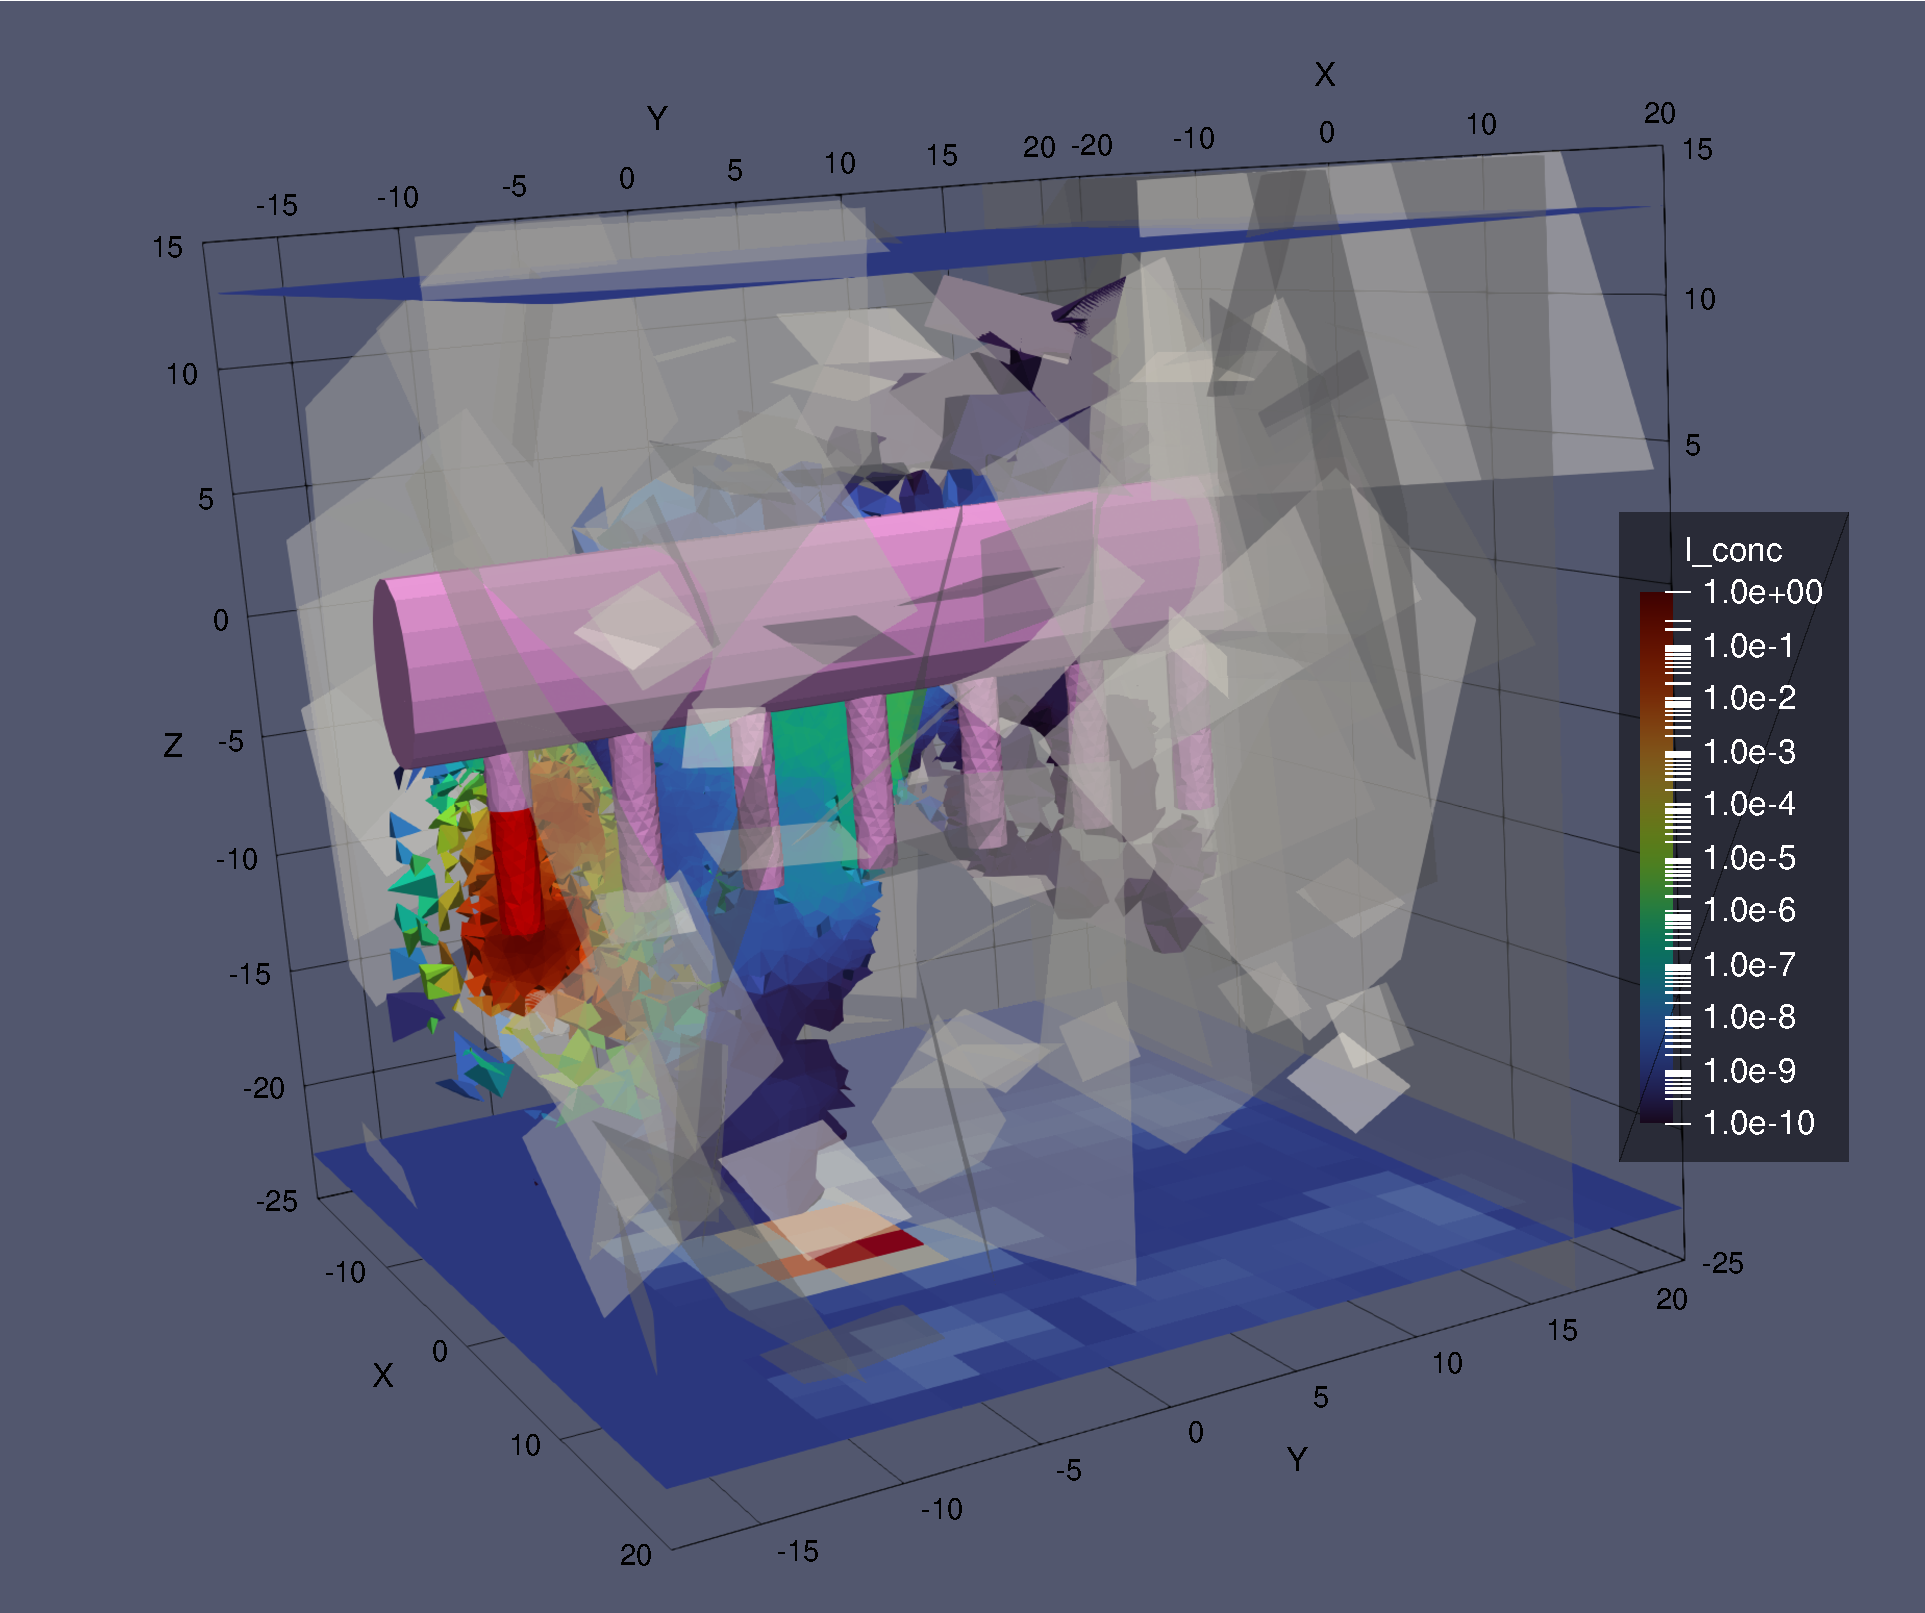
\includegraphics[width=0.75\textwidth]{graphics/tr/conc_cloud_001.pdf}
\caption{Example of the stochastic \gls{DFN} (transparent gray planes) in the
computational domain at simulation time $500\,\munit{y}$. The concentration
cloud is displayed in logarithmic color scale, together with the evaluation
planes near the top and bottom boundaries.}
\label{fig:conc_cloud_fractures}
\end{figure}

\subsection{Advection-diffusion equations}
Contaminant transport is caused by groundwater flow, which is described by the
continuity equation and Darcy's law for low velocities. For long-term
steady-state conditions, the stationary form of the flow equations can be
considered as:
\begin{equation}
    \label{eq:darcy_matrix}
    \div \vc v = 0, \quad \vc v = -\tn K \grad (p + z),
\end{equation}
where $\vc v$ $\bunit{m\cdot s^{-1}}$ is the Darcy (macroscopic) flow
velocity, $\tn K$ $\bunit{m\cdot s^{-1}}$ is the hydraulic conductivity tensor,
$p$ $\bunit{m}$ is the pressure head, and $z$ $\bunit{m}$ is the vertical
component of the position vector. When modeling transport through the EDZ, the
hydraulic conductivity tensor, which can be significantly heterogeneous and
anisotropic, plays an important role.
% The influence of the EDZ on $\tn K$ will be described in Chapter \ref{sec:poroelasticity} using the poroelastic model.

After solving the equation \eqref{eq:darcy_matrix} with suitable boundary
conditions and obtaining the velocity field $\vc v$, the time evolution of the
concentration of the conservative tracer $c$ $\bunit{kg\cdot m^{-3}}$ can be
described by the advection-diffusion equation:
\begin{equation}
   \label{eq:transport_matrix}
   \prtl_t (\theta c) + \div(\vc j) = f_w,\quad
   \vc j = \vc v c - \theta \tn D \grad c,
\end{equation}
where $\theta$ $\bunit{-}$ is the porosity, $\tn D$ $\bunit{m^2\cdot s^{-1}}$
is the diffusion and hydrodynamic dispersion tensor, hereafter referred to as
the {\it dispersion tensor}. Diffusion is due to the chaotic motion of solution
molecules, while dispersion is due to velocity field inhomogeneity at the
microscopic level.
% , see  Section \ref{sec:transport_multiscale}.
For the case of an isotropic medium, the dispersion tensor is given:
\begin{equation}
  \label{eq:dispersion_tn}
  \tn D = \tn D_e + \abs{\vc u}\Big(\alpha_T \tn I + (\alpha_L - \alpha_T)\frac{\vc u \otimes \vc u}{\abs{\vc u}^2}\Big),
\end{equation}
where
\begin{itemize}
 \item $\tn D_e = d_e \tn I$ is the molecular diffusion tensor, which for
 simplicity, we consider to be isotropic with a~coefficient of effective
 diffusion $d_e$ $\bunit{m^2\cdot s^{-1}}$, on the order of $10^{-9}$ for pure
 water,
%$[-]$ is the tortuosity according to \cite{millington_permeability_1961},
 \item $\alpha_L$ and $\alpha_T$ $\bunit{m}$ are the longitudinal and
 transverse dispersion coefficients,
 \item $\vc u$ is the pore velocity, $\vc u = \vc v / \theta$.
\end{itemize}

The contaminant volumetric source $f_w$ (right hand side in
\eqref{eq:transport_matrix}) is constrained in time and space to the single
pulse in the leaking  \gls{WDP} described by  \eqref{eq:pulse_source}.

Radioactivity decay and sorption strongly influence the evolution of the
specific radionuclides' concentration. To simplify the calculations and
especially the interpretation of the results, the influence of these phenomena
is not considered in this study.
% The Flow123d simulator implements both phenomena in full generality. We show below that the simplification is acceptable for relative comparisons of WDP positions in the case of homogeneous $\theta$ porosity and sorption.

\subsection{Vector calculus for DFM}
\label{sec:vek_pocet_dfm}
The DFM setting combines processes in the rock matrix with processes on a
lower-dimensional fracture network. The resulting model is inherently
\emph{mixed-dimensional}: the governing equations live on manifolds of different
dimension and are coupled through interface terms. Most ambiguities arise in
the coupling terms (traces, normal fluxes, and sign conventions). We therefore
fix a systematic mixed-dimensional vector calculus,
following \cite{BrezinaMethodology2023} and consistent with \cite{flow123d}.
The purpose is clarity and reproducibility: once the operators and interface
mappings are set, the weak formulation and discretization follow without ad-hoc
conventions.

We denote $\Omega_m \subset \Real^3$ as the matrix region and
$\Omega_f=\Cup_{i=1}^{n_{fr}}\mathcal F_i$ as the fracture region, assuming
that the individual fractures $\mathcal F_i$ have a~polygonal shape.
%$\mathcal F_i: D_i to \Real^3$ are parametrically defined polygons.
% \sy{[Standa: For the purposes of this report, I think it is not necessary to state that fractures are parametrically defined. Also, consider introducing the notation $\Omega=\Omega_m\cup\Omega_f$, where the symbol $\Omega$ would be used for the definition of continuous models, e.g., in section 2.1, which is currently missing.]}
% \jb{It is good to realize that quantities on fractures are functions of only two parametric coordinates.}
For simplicity, we will not discuss fracture intersections further; however,
the implementation used in the Flow123d simulator accounts for them. For
a~given scalar, vector, or tensor quantity $p=(p_m, p_f)$, we denote $p_m$ as
the function of the quantity in $\Omega_m$ and $p_f$ as the function defining
the quantity in $\Omega_f$ (in fact, the function is defined on the parametric
domains $D_i$). For each point $\vc x \in \Omega_f$ on an individual fracture,
we denote $\vnu(\vc x)$ as the normal vector, also defining its orientation. We
further distinguish the positive and negative sides of the plane
$\vnu^+ = \vnu$ and $\vnu^-=-\vnu$. The quantity $p$ can be discontinuous in
the normal direction to the fracture, hence for $p_m$, we define its value on
the sides of the fracture: $p_m^+$, $p_m^-$. The fracture thickness field is
denoted as $\delta(\vc x)$.

To simplify the notation of equations on fractures, we now introduce
semi-discrete differential operators. For a~scalar quantity $p$, $p_f$ is
a~function of two variables, and its tangential gradient $\grad_t p_f$ is
a~tangential vector to $\Omega_f$. The semi-discrete gradient then approximates
the normal component using the difference of traces:
$$
\fgrad p = \grad_t p_f + \grad_\nu p,\qquad
\grad_\nu p = \frac{1}{2}\Big(\Delta^+ p\vnu^+  + \Delta^- p\vnu^-\Big),
$$
where the normal component is approximated by the sum of differences across the
sides of the fracture:
$$
\qquad \Delta^\pm p = \frac{2}{\delta}\Big(p_m^\pm - p_f\Big).
$$
We further define the semi-discrete gradient on the positive and negative sides
of the fracture plane:
$$ \fgrad^\pm p = \grad_t p_f + \Delta^\pm p\vnu^\pm. $$
This definition allows the formal extension of notation for fracture
intersections.
% \todo{It appears that equations can indeed be written with these summed operators, but for the writing of the Neumann boundary condition, which forms the link, we still need to introduce $\fgrad^\pm$.}

In the same manner, we introduce the gradient for a~vector field
$\vc v=(\vc v_m, \vc v_f)$:
$$
\fgrad \vc v = \grad_t \vc v_f + \grad_\nu \vc v,\qquad
\grad_\nu \vc v = \frac{1}{2}\Big(\Delta^+\vc v \otimes\vnu^+  + \Delta^- \vc v\otimes\vnu^-\Big),
$$
Similarly, we then introduce the semi-discrete divergence of a~vector field:
$$
\fdiv \vc v = \div_t \vc v_f + \div_\nu \vc v,\qquad
\div_\nu \vc v = \frac{1}{2}\Big(\Delta^+ \vc v \cdot \vnu^+  + \Delta^- \vc v \cdot \vnu^-\Big)
$$
Here, the tangential divergence $\div_t \vc v_f$ is the divergence of the
tangential component of the field $\vc v_f$. Similarly, we introduce the
divergence for a~tensor quantity $\vc\sigma = (\vc\sigma_m, \vc\sigma_f)$:
$$
\fdiv \vc\sigma = \div_t \vc\sigma_f + \div_\nu \vc\sigma,\qquad
\div_\nu \vc\sigma = \frac{1}{2}\Big(\Delta^+ \vc\sigma \vnu^+  + \Delta^- \vc\sigma \vnu^-\Big).
$$

\subsection{Transport equations for DFM description}
\label{sec:transport_DFN}

For the DFM description, equation \eqref{eq:darcy_matrix} is considered only in
the matrix region $\Omega_m$. In the fracture network $\Omega_f$, the flow is
described by the equation:
\begin{equation}
    \label{eq:darcy_fracture}
    \fdiv (\delta \vc v_f) = 0, \quad \vc v_f = -\tn K_f \fgrad (p + z).
\end{equation}
Here, $\tn K_f(\vc x)$ is the 3D conductivity tensor describing the material of
the fracture network. The coupling between the regions is given by the balance
of volumetric flux at the interfaces between the matrix and the fracture, which
represents a~Neumann boundary condition for equation \eqref{eq:darcy_matrix} on
$\Omega_m$. A~separate condition must be considered for each side of the
fracture:
\begin{equation}
    \vnu^{\pm} \cdot \vc v_m^\pm = \vnu^{\pm} \cdot \vc v_f^\pm =
    -\vnu^\pm \cdot \left(\tn K_f \fgrad^\pm (p + z)\right)
    \quad \text{on }\Omega_f.
\end{equation}
For the flow model, we consider a~Dirichlet boundary condition for the
piezometric head $P = p + z$, which is interpolated from the regional flow
model at the model location.

Similarly, for the DFM description of transport, we consider
equation \eqref{eq:transport_matrix} only for the matrix $\Omega_m$,
while in the fractures $\Omega_f$, the transport equation takes the form:

\begin{equation}
   \label{eq:transport_fr}
   \prtl_t (\delta\theta c_f) + \fdiv \,\vc j = 0, \quad
   \vc j_f = \vc v_f c_f - \delta \theta \tn D \fgrad c.
\end{equation}
The coupling between the regions, similar to flow, is given by the balance of
the tracer mass flux:
\begin{equation}
    \vnu^{\pm} \cdot \vc j_m^\pm  = \vnu^{\pm} \cdot \vc j_f^\pm
    \quad \text{on }\Omega_f.
\end{equation}
At the outer boundary of the model, a~zero mass flux is considered at the
inflow part of the boundary, and a~zero diffusive flux is considered at the
outflow part of the boundary.

\def\rmin{\underline r}
\def\rmax{\overline r}
\subsection{Stochastic model of fracture network}
As Darcy flow in crystalline rock is primarily attributed to fractures,
discrete fracture network (DFN) models are commonly employed by
\cite{deDreuzy2012Influence}. Our DFM approach applies the same stochastic
model of the fractures, where, however, just a small range of the largest
fractures is discretized explicitly, while smaller-scale fractures are
represented by upscaled heterogeneous material fields. In particular, we adopt
the DFN parametrization from SKB report by \cite{Ohman_Site_2010}.
\begin{enumerate}
\item Based on evidence from nature, \cite{Bonnet_Scaling_2001}, we assume a
truncated power-law distribution of the fracture sizes:
\begin{equation}
    \label{pow_law}
    f_s \sim C r^{-\alpha},
    \qquad
    C = \frac{1-\alpha}{\rmax^{1-\alpha} - \rmin^{1-\alpha}},
\end{equation}
where $\alpha$ represents the characteristic exponent, while $\rmin$ and
$\rmax$ denote the minimum and maximum lengths of a fracture, respectively. The
$\rmin$, $\rmax$ are rather arbitrary parameters providing a scale window where
the power-law is assumed.

\item Poisson process is assumed for the centers of the fractures. The density
parameter
$P_{32}$  $[m^{-1}]$ is the average total surface area of the fracture of size
$r\in(\rmin, \rmax)$ within a unit volume. Alternatively, dimensionless and
scale-independent density could be used to better describe the connectivity of
DFN, see \cite{Adler1999} for details.

\item
The distribution of orientations is modeled by Fisher distribution. Five
families of fractures with significantly different orientations are considered.

\item We adopt the power-law model for fracture transmissivity from
\cite{Ohman_Site_2010} in a dimensionless form,
\[
    T = \delta K_f = a\left(\frac{r}{r_0}\right)^{b},
\qquad r_0 = 1\,\mathrm{m},
\]
where $T$ is the fracture transmissivity $[\,\mathrm{m^2\,s^{-1}}\,]$, $\delta$
is the hydraulic aperture
$[\,\mathrm{m}\,]$, $K_f$ is the fracture hydraulic conductivity
$[\,\mathrm{m\,s^{-1}}\,]$, and $r$ is the fracture radius
$[\,\mathrm{m}\,]$.

Using the cubic law with a constriction factor $f_K$ $[-]$,
\begin{equation}
    \label{eq:k_frac}
    K_f = f_K \frac{g \rho_w}{12\mu}\,\delta^{2},
\end{equation}
where $g$ is the gravitational acceleration $[\,\mathrm{m\,s^{-2}}\,]$,
$\rho_w$ is the water density $[\,\mathrm{kg\,m^{-3}}\,]$, and
$\mu$ is the dynamic viscosity of water $[\,\mathrm{Pa\,s}]$.
Substituting \eqref{eq:k_frac} into $T=\delta K_f$ yields
aperture:
\begin{equation}
    \label{eq:k_frac_1}
    \delta = \alpha \left(\frac{r}{r_0}\right)^{\beta},
    \qquad
    \alpha = \left(\frac{12\mu\,a}{f_K g \rho_w}\right)^{\!1/3},
    \qquad
    \beta = \frac{b}{3}.
\end{equation}
Here $\beta$ is dimensionless and $\alpha$ has units $[\,\mathrm{m}\,]$, as
expected for an aperture.

\end{enumerate}

For simplicity, we assume uncorrelated fractures with positions determined by a
Poisson process and independent orientations. See
\cite{Sahimi20110420, Liu2016} for more general models.
% Additionally, we consider the cubic law for fracture hydraulic conductivity:

\subsection{Boundary conditions}
\jb{Rather move to parameterization section.
}
The steady Darcy flow is driven by a Dirichlet boundary condition imposed on
the outer boundary of the bulk domain. We prescribe a homogeneous gradient of
the piezometric head,
\[
p(x,y,z) = 0.05\,(-y + 0.1z),
\]
which induces a gently decreasing mean velocity field parallel to the tunnel
(in $y$  direction). The resulting velocity magnitude is on the order of
$10^{-11}$, comparable to the groundwater velocity at the repository domain in
the hydrological model of the test locality \textquote{Kraví hora}. To avoid
unrealistically high fluxes along fractures (in particular the large collecting
fracture), we exclude fractures from the boundary condition enforcement.

The advection--diffusion equation is driven by an inflow boundary condition: the
diffusive flux is set to zero on the entire boundary, and the concentration is
set to zero on the inflow portion. Because the problem is diffusion-dominated,
the zero diffusive-flux condition can be viewed as a conservative
approximation, as it prevents outward diffusive loss and thus tends to increase
the resulting concentration of the safety indicator.

\subsection{Heterogeneous fields}
\label{sec:parameters}

The model includes matrix parameters defined as spatially variable fields. Rock
and bentonite are represented as separate domains. Bentonite is treated as
relatively homogeneous, whereas the rock mass is heterogeneous due to
(i) excavation-induced effects caused by stress redistribution and
(ii) sub-element-scale fractures that introduce random variability. We address
the former via \gls{EDZ} parametrization; the latter requires a non-Gaussian
stochastic representation and is the subject of ongoing research.

\def\edzRelThick{{\color{red}\tilde{w}_e}}
\def\edzPerm{{\color{red}\tilde{k}_e}}
\def\iPerm{{\color{blue}k_r}}
\def\edzPor{{\color{red}\tilde{\theta}_e}}
\def\iPor{{\color{blue}\theta_r}}

\paragraph{EDZ fields}
\jb{Need to remove reference to the HM modelling of excavation.}

In Section \ref{sec:hm_steady}, we study the expected permeability changes
induced by excavation. However, because the homogeneous model used there does
not match the experimental data described in Chapter \ref{ch:inversion}, we
neglect the potentially significant angular variability associated with the
orientation of the maximum initial stress. Instead, we adopt a simplified model
that considers only radial variability, and we use the permeability range
predicted by the HM model to prescribe uncertainty (discussed later in
Section \ref{sec:parameters}).

The scalar permeability $k(\vc x)$ is interpolated on a logarithmic scale
(i.e., using geometric progression) between the most perturbed permeability
$k_e=\edzPerm\,\iPerm$ at the tunnel wall and the intact rock permeability
$\iPerm$ at the outer boundary of the EDZ:
\begin{equation}
    \label{eq:edz_perm}
    \log k(\vc x) = (1-t)\,\log(k_e) + t\,\log(\iPerm),
    \qquad
    t=\frac{d(\vc x)-1}{\edzRelThick-1}.
\end{equation}
Here $d(\vc x)$ denotes the distance from the tunnel axis, normalized by the
tunnel radius, so that $d=1$ at the tunnel wall. The parameter $\edzRelThick$
defines the outer boundary of the EDZ as a multiple of the tunnel radius.

Similarly, we prescribe the spatially variable porosity as
\begin{equation}
    \label{eq:edz_por}
    \theta(\vc x) = (1-t)\,\theta_e + t\,\theta_r,
    \qquad
    \theta_e = \edzPor\,\iPor.
\end{equation}

The red parameters $\edzRelThick$, $\edzPerm$, and $\edzPor$ characterize the
EDZ, while the blue parameters correspond to intact rock.

\paragraph{Dispersion}
Dispersion is an apparent spreading caused by spatial variability in the
velocity field, which in turn reflects heterogeneity in permeability. Although
we do not explicitly model random spatial heterogeneity in the conductivity
(permeability) field, its macroscopic effect can be represented through an
effective dispersion.

Using first-order stochastic theory for macroscopic dispersion
\cite{Zech_Evidence_2023}, the longitudinal dispersivity is proportional to the
variance of $\ln K$ and to the integral scale $I_h$:
\begin{equation}
    \alpha_L = \sigma_{\ln K}^2\, I_h .
\end{equation}
In our case, we take $\sigma_{\ln K}^2$ to be the same variance used to
represent uncertainty in the bulk permeability. The integral scale is bounded
above by the characteristic size of the largest unresolved fractures
(approximately $5\,\mathrm{m}$) and below by the mesh size
(approximately $0.5\,\mathrm{m}$). Following a common rule of thumb, we set the
transverse dispersivity to one tenth of the longitudinal value.

\subsection{Numerical scheme and HPC computation}
\jb{Shorten or eliminate this section.}

The numerical simulations of flow and transport are performed with the
\emph{Flow123d} software. The Darcy flow equations \eqref{eq:darcy_matrix} and
\eqref{eq:darcy_fracture} are discretized by a mixed--hybrid finite element
method: the velocity field is approximated using lowest-order Raviart--Thomas
(RT0) elements, while the pressure head is represented by piecewise-constant
 elements. Flux continuity across element interfaces is enforced by Lagrange
multipliers defined on element faces. The computational mesh consists of
simplices, and it is constructed so that 2D fracture elements coincide with
faces of the adjacent 3D bulk elements. The resulting discrete problem can be
written in the block form:
\begin{equation}
\label{eq:flow_alg_mh}
\begin{bmatrix}
\tn A_{\vc v\vc v} & \tn B_{\vc v p} & \tn B_{\vc v\lambda}\\
\tn B_{\vc v p}^\top & \tn O & \tn O\\
\tn B_{\vc v\lambda}^\top & \tn O & \tn O
\end{bmatrix}
%
\begin{bmatrix}
\uu^{\vc v}\\
\uu^p\\
\uu^\lambda
\end{bmatrix} =
%
\begin{bmatrix}
\vc 0\\
\vc f^p\\
\vc 0
\end{bmatrix},
\end{equation}
where $\uu^{\vc v}$, $\uu^p$, and $\uu^\lambda$ denote the degrees of freedom
associated with the velocity field, the pressure head at mesh element
centroids, and the Lagrange multipliers, respectively. The vector $\vc f^p$
represents the discrete source term in the mass balance. The matrices
$\tn A_{\vc v\vc v}$ and $\tn B_{\vc v p}$ are assembled only locally on an
element-by-element basis, which allows for an efficient per-element
construction of the Schur complement. Consequently, the saddle-point system
\eqref{eq:flow_alg_mh} can be reduced to a system for $\uu^\lambda$ with a
symmetric positive definite matrix, which is solved using a CG method with an
algebraic multigrid preconditioning.

The transport equations \eqref{eq:transport_matrix} and \eqref{eq:transport_fr}
are discretized using the discontinuous Galerkin method (DGM), typically with
first- or second-order polynomial approximation. To improve robustness across a
wide range of advection-to-diffusion ratios, we employ a non-symmetric DGM
variant, which leads to a nonsymmetric algebraic system. solved using the GMRES
method with ILU preconditioning.

This section introduces the grouped Sobol framework used for the sensitivity
analysis, then specifies the stochastic distributions of the model parameters,
and finally interprets the simulation results. In the results part, we first
summarize transport features common to all cases, namely the role of dispersion
and the advection-to-diffusion balance, and only then discuss the individual
case studies.
